\documentclass[a4paper,times,10pt,authoryear]{article}%

\usepackage[top=1in,left=1in]{geometry}
\usepackage{url}
\usepackage{natbib}
\usepackage{graphicx}
\usepackage{setspace}

\usepackage{lineno}
\linenumbers

\doublespacing 

\begin{document}


\title{1) How to improve PCA based methods of genome scan using ecological data: detecting selection using RDA. \\ 2) How to make use of ordination methods in landscape genomics studies: a comparison of PCA and RDA approaches \\  3) How to improve ordination based methods of genome scan using ecological data: a comparison of PCA and RDA approaches for the detection of outliers.}

\maketitle


\author{Eric Bazin,$^{\ast,1}$ Keurcien Luu,$^{2}$ Michael G. B.
Blum,$^{2}$}

$^{1}$LECA, Universit\'{e} de Grenoble - $^{2}$TIMC, Universit\'{e} de Grenoble

E-mail: eric.bazin@univ-grenoble-alpes.fr



\begin{abstract}
Ordination is a common tool in Ecology that aims at representing complex biological information on a reduced space. For instance, it is frequently used to study geographic distribution pattern of species diversity and to study the link between ecological variable such as temperature, drought, etc, on the species turnover. 
Recently, ordination methods such as PCA have been used as a framework to detect genes under selection. Simulations support this idea has it is quite robust to the underlying population structure and dynamic. Some authors have proposed to use other ordination approaches  such as RDA (i.e. Redundancy analysis), taking advantage of using environmental data. However no clear statistical framework have been developed to efficiently implement this latter idea in a robust and efficient test and it hasn't been tested on demogenetic simulations either.
Furthermore, these methodologies are becoming quite popular in Landscape Genomic where one wants to study the link between environmental variable and the distribution pattern of genome wide diversity especially its adaptive component. However, it remains unclear what are the expected outcome of such approaches since genetic diversity has presumably a very different dynamic from species diversity. Whereas it tends to be broadly accepted as a pertinent approach, a validation by simulations studies is still lacking. 
This paper aims at proposing a new test based on RDA approaches to search for genes under selection and to compare it to a classical PCA method. Thanks to individual based simulation, we show that RDA genome scan has greater power than PCA genome scan to detect true positives. Additionally, we show that RDA is efficient to point out relevant selective gradient among the different environmental variables. Finally, to illustrate the pertinence of such method in concrete example, we apply it to a real dataset.
\end{abstract}





\section{{Introduction}\label{sec:Intro}}

\subsection{Context}
Natural selection is the result of a complex set of environmental pressures. It most often acts on several characters simultaneously and these characters are encoded by several genes which generally have weak effects. Patterns of adaptive variation within species are usually studied through physiological, morphometric and fitness comparisons in common gardens experiments. However, this is a difficult and constraining task and is even unrealistic on species with long generation time. The recent development of Next Generation Sequencing (NGS) technics has opened the possibility to access to a large amount of genetic variation across the genome. Therefore, the link between genetic polymorphism, phenotypic variation and environmental variables can now be studied and quantified by in situ approaches.

The search of adaptive genetic variation can be performed by genome scan methods, a common task in population genomic area \citep{Foll2008,Frichot2013,Luu2016,Vatsiou2015}. Some methods aim at detecting  genes that has suffered from a loss of genetic diversity and increase of linkage disequilibrium following the appearance of a beneficial allele and its spread by the mean of selective sweep. Others aim at picking up alleles with strong correlation with some environmental variable (e.g. Temperature, drought) with the idea that these alleles may confer a selective advantage to the individuals  \citep{Coop2010,Frichot2013}. Finally, other methods aim at detecting genomic region involved in local adaptation process. These region should have an increased differentiation between population because different alleles tend to be beneficial in each environment. Differentiation between population is excepted under the hypothesis of geographical isolation. Therefore, this region can be detected by quantifying the level of differentiation using some statistics and detecting the regions with unexpectedly high values. A common statistic and very easily comprehensible in population genetic is $F_{ST}$. Many methods use this parameter as a basis in many different implementation of genome scans \citep{Bazin2010,DeVillemereuil2015,Foll2008}. These are model based method where parameters such as $F_{ST}$ are usually inferred using likelihood or Bayesian methods. This mean that users must have some a priori on their parameter value and the best model that fits their data in order to expect the best from their analysis.

However, it is often difficult to get a satisfactory a priori picture of the demographic and population structure of the species one is interested in. Indeed many species are not clearly structured in different populations but more or less show a pattern of isolation by distance without clear geographical barrier to gene flow. One solution would be to use more complex model that better reflect reality but these are difficult to implement in Bayesian framework. Additionally, these latter methods are very time consuming and the increase of both model complexity and the amount of data to analyze in terms of the number of individuals and loci makes them more and more difficult to use.

A new path has opened recently with the use of multivariate methods. The idea is to capture the whole genome geographic structure using an ordination method such as ACP. Following this analysis, outliers loci are detected if they have extremely high correlation with one or more ordination axis \citep{Duforet-Frebourg2014a,Luu2016}.  These are very efficient methods and simulations have shown that while they are very fast, they show similar efficiency than classical Bayesian method and sometimes perform better when the simulated demographic model drift from the model implemented in bayesian method, usually the island model. For instance \citet{Luu2016} have shown their method to be better when population are structured in hierarchical set or in isolation by distance pattern. Nevertheless, one conundrum of such approaches is the difficulty to interpret ordination axis in term of ecological meanings. These are usually tight to geographical axis (latitudinal or longitudinal) but they are not necessary linked to an environmental variable such as Temperature, drought, diet habit, etc. Therefore, when this information exists, it has to be a posteriori used as a mean of interpretation but are not involved in the inference process.

However, thanks to the improvement of genome scan technics, it is now feasible to detect the adaptive fraction among the whole genetic variation. Some authors \citep{DeKort2014,Steane2014a} have proposed to use ordination technics such as RDA (Redundancy Analysis) or CAPs (Canonical Analysis of Principal coordinates) to subsequently align the adaptive variation with environmental data in order to be able to identify the environmental gradient that are the most correlated to the adaptive variation. This can even be used to derive adaptive index that predict the performance of individuals in different environmental which is analogous to the adaptive variation that is measured in common garden experiments. For instance, \citet{Steane2014a} had applied this approach on \textit{Eucalyptus trichocarpa} populations and shown that this {in-situ} estimation of adaptive variation is correlated to what can be measured in common garden experiments.

%In order to extract the maximum of all available information, it seems therefore necessary to use approaches that are able to compile all kind of variable (e.g. alleles, phenotypic measurement, biotic and abiotic variables).

For all these reasons, the use of multivariate methods are becoming popular in population genomic studies both to perform genome scans and to quantify multilocus adaptation to an environmental gradient \citep{Lasky2012,DeKort2014,Steane2014a,Hecht2015}. These studies whereby relationships between environmental data and large multilocus data is explored are often coined as Ecological Genomics or Landscape Genomics studies.
	

\subsection{Content}

One natural way to overcome the limitation of actual genome scan methods due to the complexity of date (e.g. alleles, phenotypic measurement, biotic and abiotic variables) would be to use more sophisticated ordination method than ACP like methods. Constrained ordination methods (i.e. Redundancy Analysis, RDA, Canonical Analysis of Principal coordinates, CAP) are well-known set of approaches in Ecology for instance to explain the species distribution pattern by the mean of environmental data. They have specifically been designed in order to deal with biological complexity. In the population genomic era, it appears that data amount, complexity and heterogeneity is often a limitation to the use of inference methods based on classical population genetic models. Although they are more difficult to interpret, such approaches would be complementary to the model based method because of their long-term use in ecology and their efficiency on complex and large datasets. 

In this paper, we show how one can make use of a constrained ordination method namely Redundancy Analysis (RDA) as an efficient and robust genome scan method. We discarded the other constraint ordination methods such as CAPs since they are very similar in their principles. RDA has already been used for instance by \citet{Lasky2012} to perform genome scan in order to detect loci involved in the adaptation to climate in \textit{Arabidopsis thaliana}. Outliers were identified as SNPs with the greatest squared scores along the first RDA axis (i.e. those in the 0.5 \% tail). We build on this idea to develop a comprehensive and robust statistical test for searching loci under selection. 

Furthermore, even if common garden experiments seem to validate the use of ordination technics such as RDA to identify selective gradient linked to adaptive variation \citep{Steane2014a} among the environmental variables, this idea has never been tested thoroughly on simulated data sets. It would however shed light on the conditions within which the approach is the most efficient. This paper aims at filling this gap by performing demogenetic simulations with selection determined by different environmental gradient acting on traits coded by several loci.

	
\subsection{Conclusion}	
	
First, when applied to the simulated data, we show that our RDA based genome scan allows to recover more outliers than blind PCA based method by taking into account environmental variable and that it allows to control precisely for the false discovery rate. 

Second, thanks to our simulations, we show that RDA can indeed help to identify important environmental gradient that better explain the adaptive variation in the data. It is therefore a proof of concept of the idea of using constrained ordination method as an environmental genomic tool to identify relevent selective gradient in the environmental data as this was proposed by \citet{DeKort2014,Steane2014a} for instance. 

Finally, to give a concrete illustration of RDA approach in population genomics, we apply this method to the detection of outliers and selective gradients on a real data set.


\section{Material and method}

\subsection{Genome scan}

Redundancy analysis (RDA) was first introduced by \citep{Rao1964} and is broadly described in \citep{Legendre2012} section 11.1. It is the direct extension of multiple regression to the modeling of multivariate response data. Typically the data to be analysed are separated in two sets, a response matrix Y of variable to be explained (e.g. species abundance in a set of sites; m sites and n species) and an explanatory matrix X (e.g.  a set of environmental variable within each site; m sites and p environment). 
	In the following analysis, species are replaced by loci and sites by individuals. In other word, we wish to project on a reduced space the proportion of variance in genetic difference between individuals which is better explained by environmental data.
	After this ordination, we follow the \citet{Luu2016} methodology to compute pvalues. First we compute the test statistic by regressing each of the p SNPs by the K ordination axis $X_1, ..., X_K$.

$G_j = \sum^{K}_{k=1}\beta_{jk}X_{k}+\epsilon_{j}, j=1,...,p$

where $\beta_{jk}$ is the regression coefficient corresponding to the j-th SNP regressed by the k-th ordination axis, and $\epsilon_{j}$ is the residuals vector. To summarize the result of the regression analysis for the j-th SNP, we return a vector of z-scores $z_{j} = (z_{j1}, ..., z_{jK})$ where $z_{jk}$ corresponds to the z-score obtained when regressing the j-th SNP by the k-th ordination axis.
The test statistic is a robust Mahalanobis distance D computed using covRob function of the robustR package. D should be Khi2 distributed after a correction with inflation factor (Luu et al., 2016). Pvalues are computed using K degree of freedom. We use the FDR approach to control for false positives. Qvalue are computed with qvalueR package and a loci is considered as an outlier if its qvalue is less than 10\%.
For the analysis of simulated dataset (see below), we retain the first five ordination axis to compute Mahalanobis distances as they explain most of the variance in the data. To peform the ordination, we use the 10th environmental variables as input in the explanatory matrix. In the following example, we don't use phenotypic informations since these informations are often laking in environmental genomics. Tests have shown that including phenotypic variable further improve the efficiency of RDA as a genome scan method (results not shown). Neither we use geographical coordinates which is sometimes added to control for the geographical covariation in the differentiation pattern \citep{Frichot2013}.

To emphasize the utility of RDA, we compared to pcadapt from which the idea of using multivariate method for genome scan is based. On the simulated dataset, we retain for both methods $K=5$ axis to compute Mahalanobis distances for the sake of comparison on the same dimension scale and because it explains the main amount of variance in the data using scatter plots (results not shown). To control for false positive, we used the same qvalue threshold (i.e. $\leq 10\%$).


\subsection{Environmental genomic}

Once outliers have been identified, we isolate them in a separate matrix A defining an "adaptively enriched genetic space" as coined by \citet{Steane2014a}. Following their methodology, we perform a second constrained ordination (RDA) on matrix A against environmental data. The rational of this analysis is to remove neutral variation before performing ordination in order to have a better picture of which environmental gradients have the strongest association with the adaptive genetic space. On the simulated dataset, we report the proportion of variance explained by RDA1, RDA2 and RDA3 on the "neutral variation" (i.e. the set of negative loci) and on the "adaptive variation" (i.e. the set of positive loci namely the A matrix) in order to show if they better explain the adaptive variation and if the ordination space succeed in seperating the environmental effect on different axis.


\subsection{Simulations}

To test for the efficiency of RDA in population genomic, we performed simulations using simuPop python library \citep{Peng2005}. We compared our approach to PCAdapt method to perform genome scans. Both approach are equivalent except their ordination method. Finally we use these simulations to evaluate RDA approach as a mean to detect selective environmental gradient.
	A lattice of 8x8 populations is simulated (i.e. 64 populations in total). Each population is initialized with 200 diploid individual with random genotypes. Migration is set to 0.1 so that population structure must be very smooth and genetic differentiation must show an isolation by distance pattern over the 64 populations. This is where pcadapt is best designed for. Loci are biallelic (0 or 1) like SNPs. Allele frequency of the whole population is initialized at 0.5. 1000 loci are defined. They are separated in 200 chuncks of 5 SNPs in physical linkage with recombination rate between adjacent loci fixed at 0.1. 3 different Traits are coded by a group of 10 different loci. The first trait is coded by loci 1, 11, 21, ..., 91. The trait value is simply the sum of genotype value and therefore can take value between 0 an 20. For the sake of realism, we add to each trait a random noise (non heritable variation) drawn from a normal distribution $N(0,2)$. The second trait is coded by loci 101, 111, ..., 191 and the third is coded by loci 201, 211, ..., 291. Each trait is therefore coded by free recombining SNP loci. In other words, there are 30 coding SNPs among 1000. Selection can have an effect on linked loci, for instance, loci 2, 3, 4 and 5 can be impacted by selection on locus 1. However, recombination is high enough (0.1) to expect a limited linkage effect. We have defined 10 different environmental variables. The first one determines the selective pressure on trait 1, the second one on trait 2 and the third one on trait 3. The first environment variable is a quadratic gradient coded by function  $env1 = -(\cos(\theta)*(i-3.5))^2 -(sin(\theta)*(j-3.5))^2 + 18, \theta = \pi/2$, i and j being the population indicator on the 8x8 lattice. The second one is a linear plan gradient coded by function $env2 = h*\cos(\theta)*(i-1) + h*\sin(\theta)*(j-1) + k$ with $h=2$, $\theta = \pi/4$ and $k=3$. The third environment variable simulates a coarse environment with value $env3 = 2$ for all populations except population (i,j) = {(2,2), (2,3), (3,2), (3,3), (6,2), (6,3), (7,2), (7,3), (2,6), (2,7), (3,6), (3,7), (6,6), (6,7), (7,6), (7,7)} for which $env3 = 18$. Env4, env5 and env6 have exactly the same equation than env1, env2 and env3 respectively. The remaining 4 environment variable are similar to env2 but with different value of h and $\theta$. Env7 has $h=2$, $\theta = 0$ and $k=3$. Env8 has $h=2$, $\theta = \pi/4$ and $k=0$. Env9 has $h=1$, $\theta = \pi/4$ and $k=4$. Env10 has $h=0.5$, $\theta = \pi/4$ and $k=8$. Graphical representation of mean environmental value for environment 1, 2 and 3 is given in Fig. \ref{fig:simulatedenvir}. Environment 4, 5 and 6 have respectively the same mean value spatial distribution. For a graphical representation of environment 7 to 10, see Fig. \ref{fig:environmentaldata}. Environmental equation gives a mean value of the environment variable. To avoid colinearity between environments variable, we added noise by drawing an environment value within a normal distribution $N(\mu=env, \sigma=1)$. Fitness for each trait is set to be $-e^{((x-env)^2/(2*\omega^2))}$, $x$ being the quantitative trait value, $env$ the environmental value and $\omega$ is defining selection strength and has been set to 20 which in our experience are sufficient for loci to be often detected. To get the overall fitness for a given individual, fitness associated to each trait are multiplied. Fitness are relative and selection arises on parents and determine their number of offsprings. Simulations are made across 500 generations. At the end of simulation, we sample 10 individuals per population. Therefore, we have a sample of 640 individuals with 1000 SNP-like loci.

\subsection{Real dataset}

The \textit{Populus trichocarpa} dataset is a sample of 424 individuals genotyped on 33,070 SNPs from 25 drainages (i.e., topographic units separated by watershed barriers) \citep{Geraldes2014}. Genotyping of each accession was performed as described in \citep{Geraldes2013} using a 34K Populus SNP array targeting 34,131 SNPs mostly within (plus 2kb upstream and downstream) 3543 genes. Details of SNP and gene selection can be found in \citep{Geraldes2013}. 21 climatic variables are available on each sampling site (details in Table S1). For the RDA and pcadapt analysis, we retained respectively $K=6$ (Fig \ref{fig:screeplotrda}) and $K=10$ (Fig \ref{fig:screeplotpca}) axis as they explain the majority of variance in the data. From the 33,079 SNPs, we removed the SNPs with missing values, leaving us 19,336 SNPs.


\section{Results}

\subsection{Genome scan}

When looking at the analysis on one simulation, the pcadapt method is successful at detecting QTL2 SNPs (Fig. \ref{fig:pcadapt}), is less performant at detecting QTL1 SNPs and fails entirely to pick-up QTL3 SNPs. On the other hand, RDA performs better at detecting QTL2 SNPs and retain a larger amount of the QTL1 and QTL2 SNPs (Fig. \ref{fig:rda}). Therefore, the ordination correctly detects environmental variable 1, 2 and 3 as drivers of genetical variance in the data. Over the 100 simulations, we have measured the average FDR and power for both pcadapt and RDA (Fig \ref{fig:performance}). 


\subsection{Environmental genomics}

We then performed a second RDA on the "adaptively enriched genetic space" as performed by \citet{Steane2014a} on the same simulated dataset as in Fig. \ref{fig:pcadapt} and \ref{fig:rda} and display its results on Fig. \ref{fig:rdaA}. We performed the same analyis on the 100 simulated dataset and measured the mean proportion of variance explained by the first three ordination axis and compared to the proportion of variance explained when we perform the RDA on the whole dataset. This is summarized in Fig. \ref{fig:R2}.



\subsection{\textit{Populus trichocarpa}}

Analysis of \textit{P. trichocarpa} with fdr of $0.1$ leads to a list of 105 outliers for RDA and 122 for pcadapt. Interstingly, both methods have 52 outliers in common so that 53 and 70 SNPs are outliers specific to respectively RDA and pcadapt. In total, we have detected 175 outliers loci that constitute our adaptive enriched genetic space.
When we performed the RDA analysis on the set of outliers loci as detected by pcadapt and our RDA based genome scan method, we found that the first three axis explain more variance than when the ordination was performed on all loci together (Fig. \ref{fig:varexplainedPopulus}). Furthermore, Fig \ref{fig:poplar_rda} illustrate the ordination on the first two axis from the RDA analysis performed on the A matrix.

When we compared RDA genome scan results with the outliers found by \citet{Geraldes2014} based on Fdist, bayescan and bayenv methods, we found that substential overlap between them. However, RDA based genome scan found 35 SNPs that no other methods (including pcadapt) had detected as outlier (see Table S2). 


\section{Discussion}

Fig \ref{fig:pcadapt} shows that pcadapt approach works well when the environmental gradient and the selective pressures are correlated to the  geographical pattern of isolation by distance. Whereas when the environment is a coarse environment (QTL3) it fails dramatically. Indeed, we can hypothesize that the PCA ordination in this case is not able to orientiate the genetic space differentiation into the direction of environment 3 therefore leaving no chance to detect any outliers on the QTL influenced by this environmental variable. Fig \ref{fig:rda} shows that RDA has a much better behavior than pcadapt by taking advantage of using informations of environmental local conditions. It can be attributed to a better alignment between the genetic space and the environmental variable improving the power to detect true positives.

Both methods have a good control of false discovery rate although slightly better for RDA ($12.0 \times 10^{-2}$ for pcadapt and $10.6 \times 10^{-2}$ for RDA). Results summarized on Fig \ref{fig:performance} is confirming that overall RDA shows better performance at detecting true outliers since it succeeds to detect quite often QTL1 and QTL3 SNPs. It is however less efficient at detecting QTL3 outliers but this might be due to the fact that local adaptation on a coarse environment is more difficult  that adaptation on a smooth environmental gradient as environment 1 and 2. These simulations plead in favor of using constrained ordination method instead of PCA when non genetic data such as environmental variable are available in order to orientate the axis in the direction of informative gradients.

When performing an RDA on the "adaptively enriched genetic space" A, Fig. \ref{fig:rdaA} show that the method succeed at detecting the relevant selective gradient and separating them on different axis at least on our simulation. Furthermore, Fig. \ref{fig:R2} show that the RDA applied to the A matrix explain more variance than when it is applied to the whole dataset illustrating the utility of removing neutral loci to have a better estimation of the environmental gradient effect on the adaptive variation. These simulations therefore serve as a proof of concept of \citet{Steane2014a}'s approach to represent multilocus selective gradient and the possibility to use the ordination axis it to devise a metric that provides a holistic measure of genomic adaptation. Indeed, in RDA1 is strongly associated with envir2, RDA2 with envir1 and RDA3 with envir3 whereas poorly associated with the other axis. As expected, the correlated environment are also strongly associated with this respective axis. This is reflecting the fact that in reality it is difficult on an environmental gradient to distinguish  among the covariable which one has a causal effect on the individual fitness. However, it is often sufficient for biologists when performing an exploratory analysis to identify combination of environment variable having a strong association with adaptive variation without knowing precisely the underlying mechanical process.


From the analysis of \textit{Popular trichocarpa}, we picked up some genes that can be interpreted regarding to the environmental variable. For instance, among the top SNPs, some of them are located within or nearby, POPTR\_0015s00640 implicated in cellular response to cold, POPTR\_0015s00440 involved in the regulation of circadian clock in plants. One outlier, POPTR\_0017s06840 that is not detected by pcadapt is involved in amylase catabolism, an activity that is suspected to depend of climatic conditions. Interestingly, Table S2 shows that a substantial amount of RDA genome scan outliers (35) are not detected by any other genome scan method including pcadapt. For instance, four SNPs are assigned to POPTR\_0007s04340, a dehydration-responsive protein-related which is similar to similar to early-responsive to dehydration stress ERD3 protein. However, its function remains mainly unknown. These results support the simulation analysis conclusions that RDA based genome scan is able to pick up more genes in relation to some environmental gradient than pcadapt. It is however noticeable that a large proportion of outliers are shared between PCA and RDA based methods which highlight the fact that both approaches are very similar. The lack of interpretability of PCA method is compensated by the fact that it is a blind method in regard to environmental data so it can pick up genes that we will miss using RDA because some crucial environmental data are lacking.
We can notice that there is a strong climate environmental gradient structuring the adaptive genetic space represented by RDA1. This is not surprising that so many outliers are shared between pcadapt and our RDA based genome scan method. Indeed, all climate variable are autocorrelated to the latitudinal gradient where this species has been sampled. RDA2 is not very informative as it does not clearly seperate a peculiar set of orthogonal environmental variable except PAS which stands for precipitation as snow. A substantial number of SNPs are clearly correlated to RDA1 gradient, most of them being detected by both methods. Furthermore, when looking at the proportion of variance explained by the first three axis, Fig. \ref{varexplainedPopulus} clearly confirms our simulation conclusion by showing that the adaptive genetic space is better aligned to the environmental variable then the whole genetic space. RDA1 can therefore serve as a basis to design a composite index of climate adaptation as it was proposed by \citet{Steane2014a}. This index can serve to predict (i) provenances that would perform well in the common gardens and (ii) patterns of adaptation to local climate across the geographic range.
In conclusion, although there is a large covariance between climatic variable, this analysis proves that RDA can be used to identify environmental gradients that are responsible for the adaptive differentiation across the geographic distribution of \textit{Populus trichocarpa}. This was intuitively expected but the approach is now validated on simulated datasets.
Finally, this paper shows that both methods are complementary and should be used simultaneously on the same dataset. RDA will be more easily interpretable in terms of mechanism and should pick up more genes when some important selective gradient are identified but PCA might be able to pick up outliers where no environmental data are available. However this latter method will miss outliers when selective gradient are poorly correlated to the population structure (i.e. geographical distance between populations and individuals). It is therefore crucial when performing landscape genomics to clearly characterize the environmental condition by measuring important variable that are suspected to put selective pressures on the species of interest. This can be done through RDA as it has been validated in our simulations and in the real dataset on \textit{Populus trichocarpa}. 

A myriad of constrained ordination method exist that could be used and allows to control for confounding variable (i.e. partial RDA) for instance altitude, latitude and longitude or allow to perform none linear regression between genetic and environmental data (i.e. LVM - Latent Variable Model). This is still to be tested and explored using both simulation and real data set validation.


\section{Supplementary Material}


\section{Acknowledgments}



\bibliographystyle{natbib}%%%%natbib.sty
\bibliography{Article_ca_gs}%%%refs.bib



\begin{figure*}[t]
\begin{center}
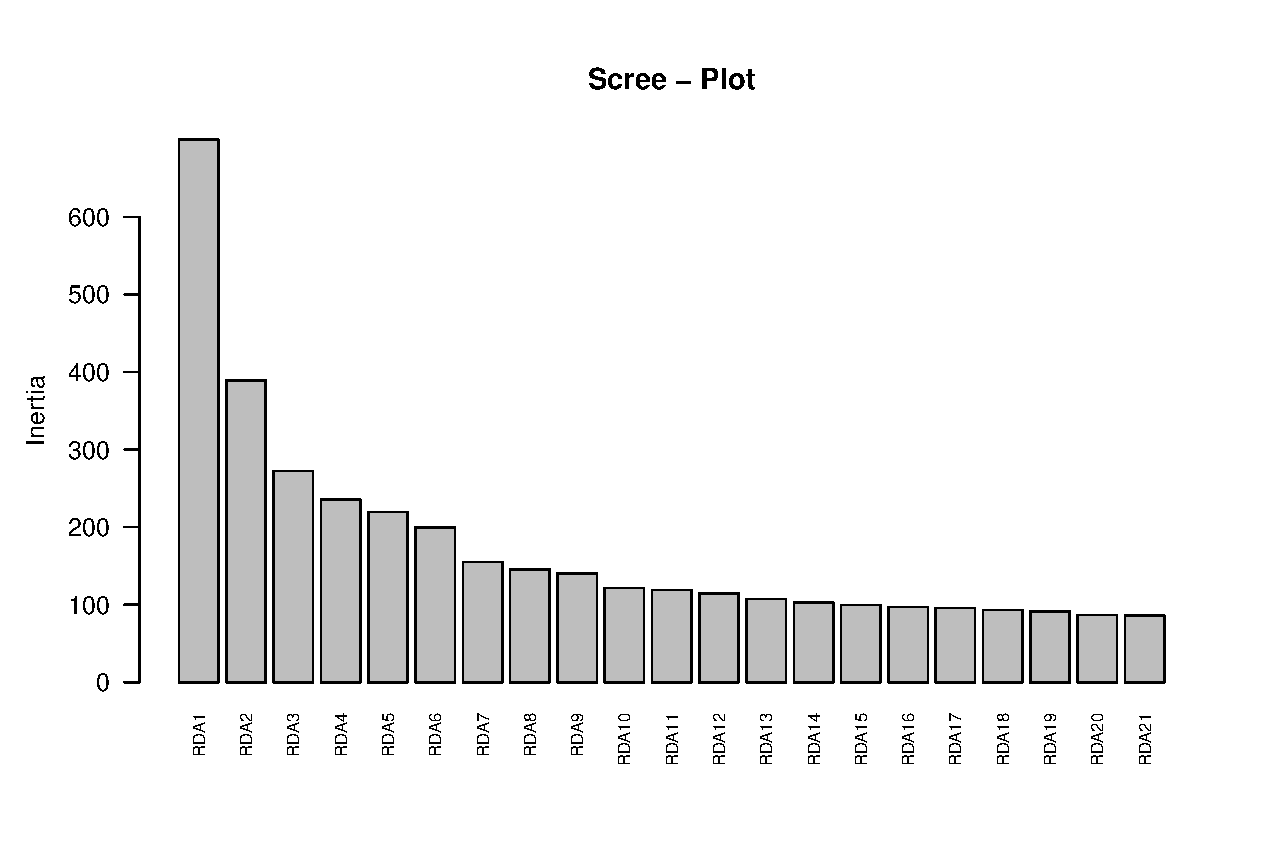
\includegraphics[height=0.25\textheight]{figures/screeplot-rda.eps}
\end{center}
\caption{Scree plot for RDA analysis of \textit{Populus trichocarpa} data}%
\label{fig:screeplotrda}%
\end{figure*}


\begin{figure*}[t]
\begin{center}
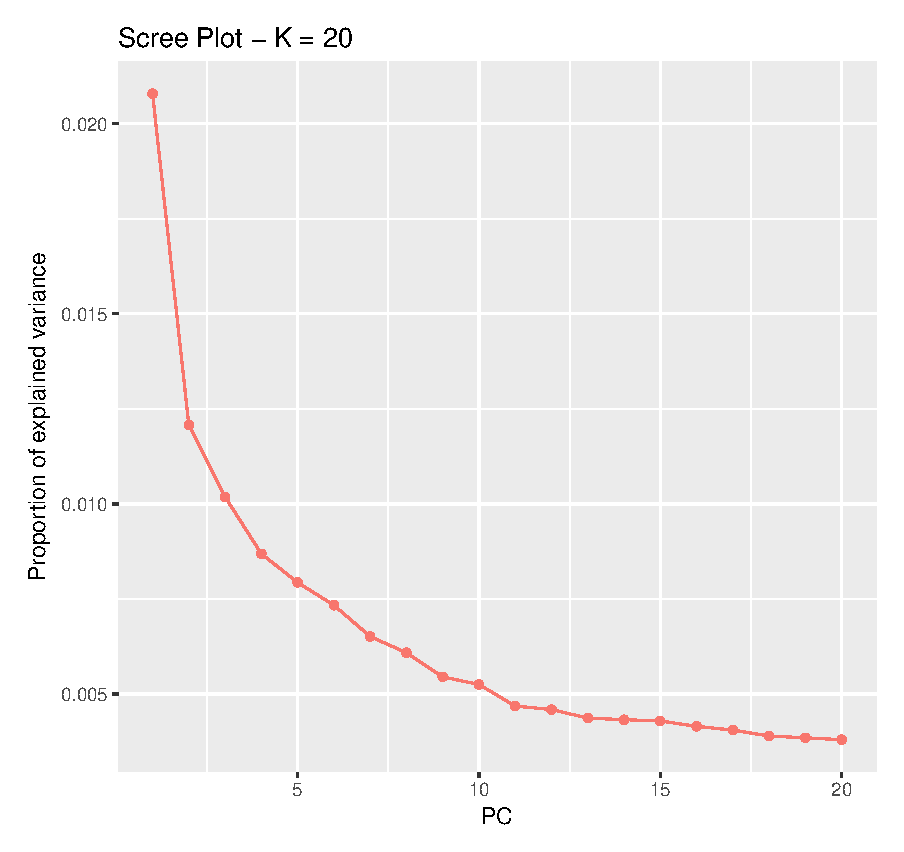
\includegraphics[height=0.25\textheight]{figures/screeplot-pca.eps}
\end{center}
\caption{Scree plot for PCA analysis of \textit{Populus trichocarpa} data}%
\label{fig:screeplotpca}%
\end{figure*}

\begin{figure*}[t]
\begin{center}
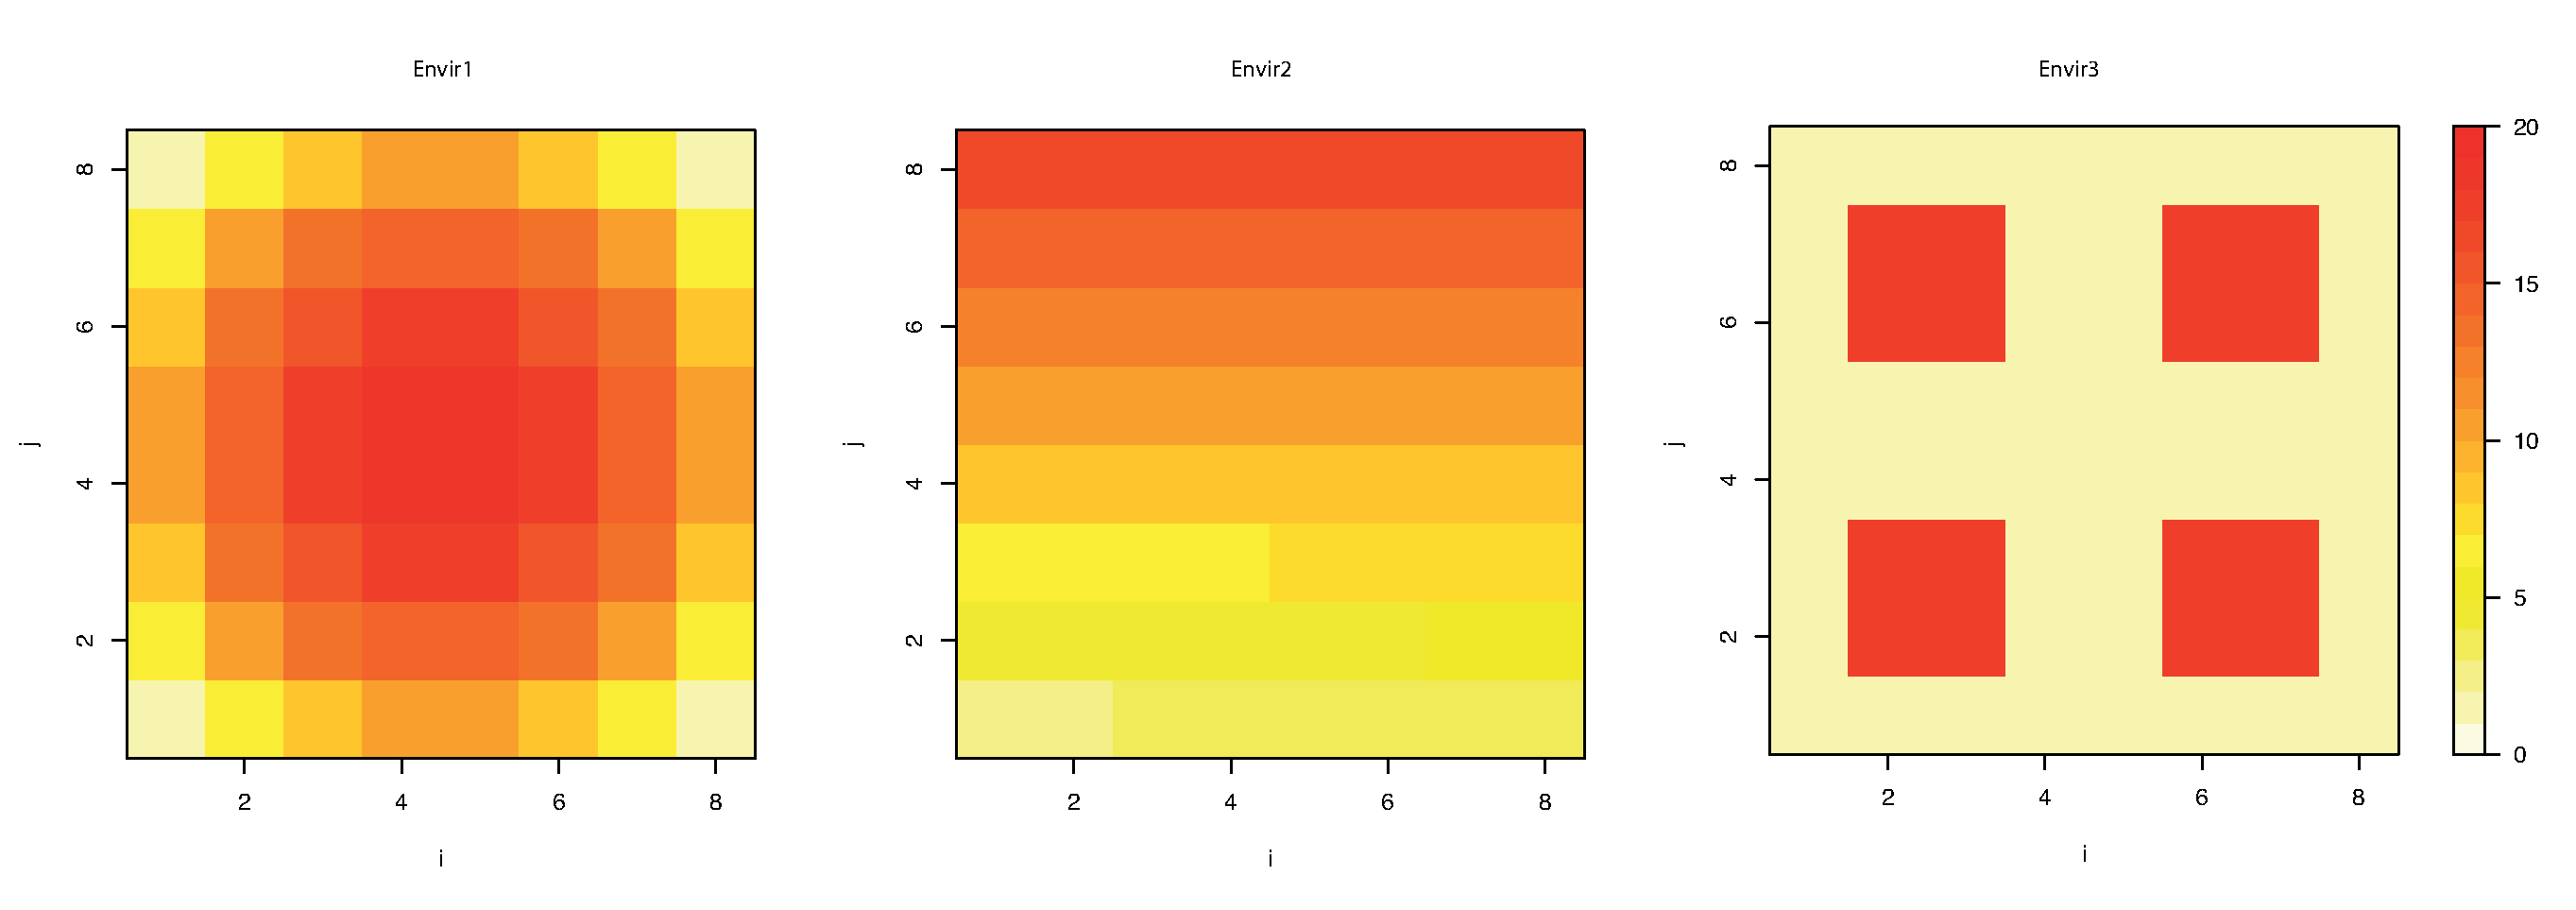
\includegraphics[height=0.25\textheight]{figures/simulatedenvironment.eps}
\end{center}
\caption{Graphical representation of mean environmental value for environment 1, 2 and 3}%
\label{fig:simulatedenvir}%
\end{figure*}

\begin{figure*}[t]
\begin{center}
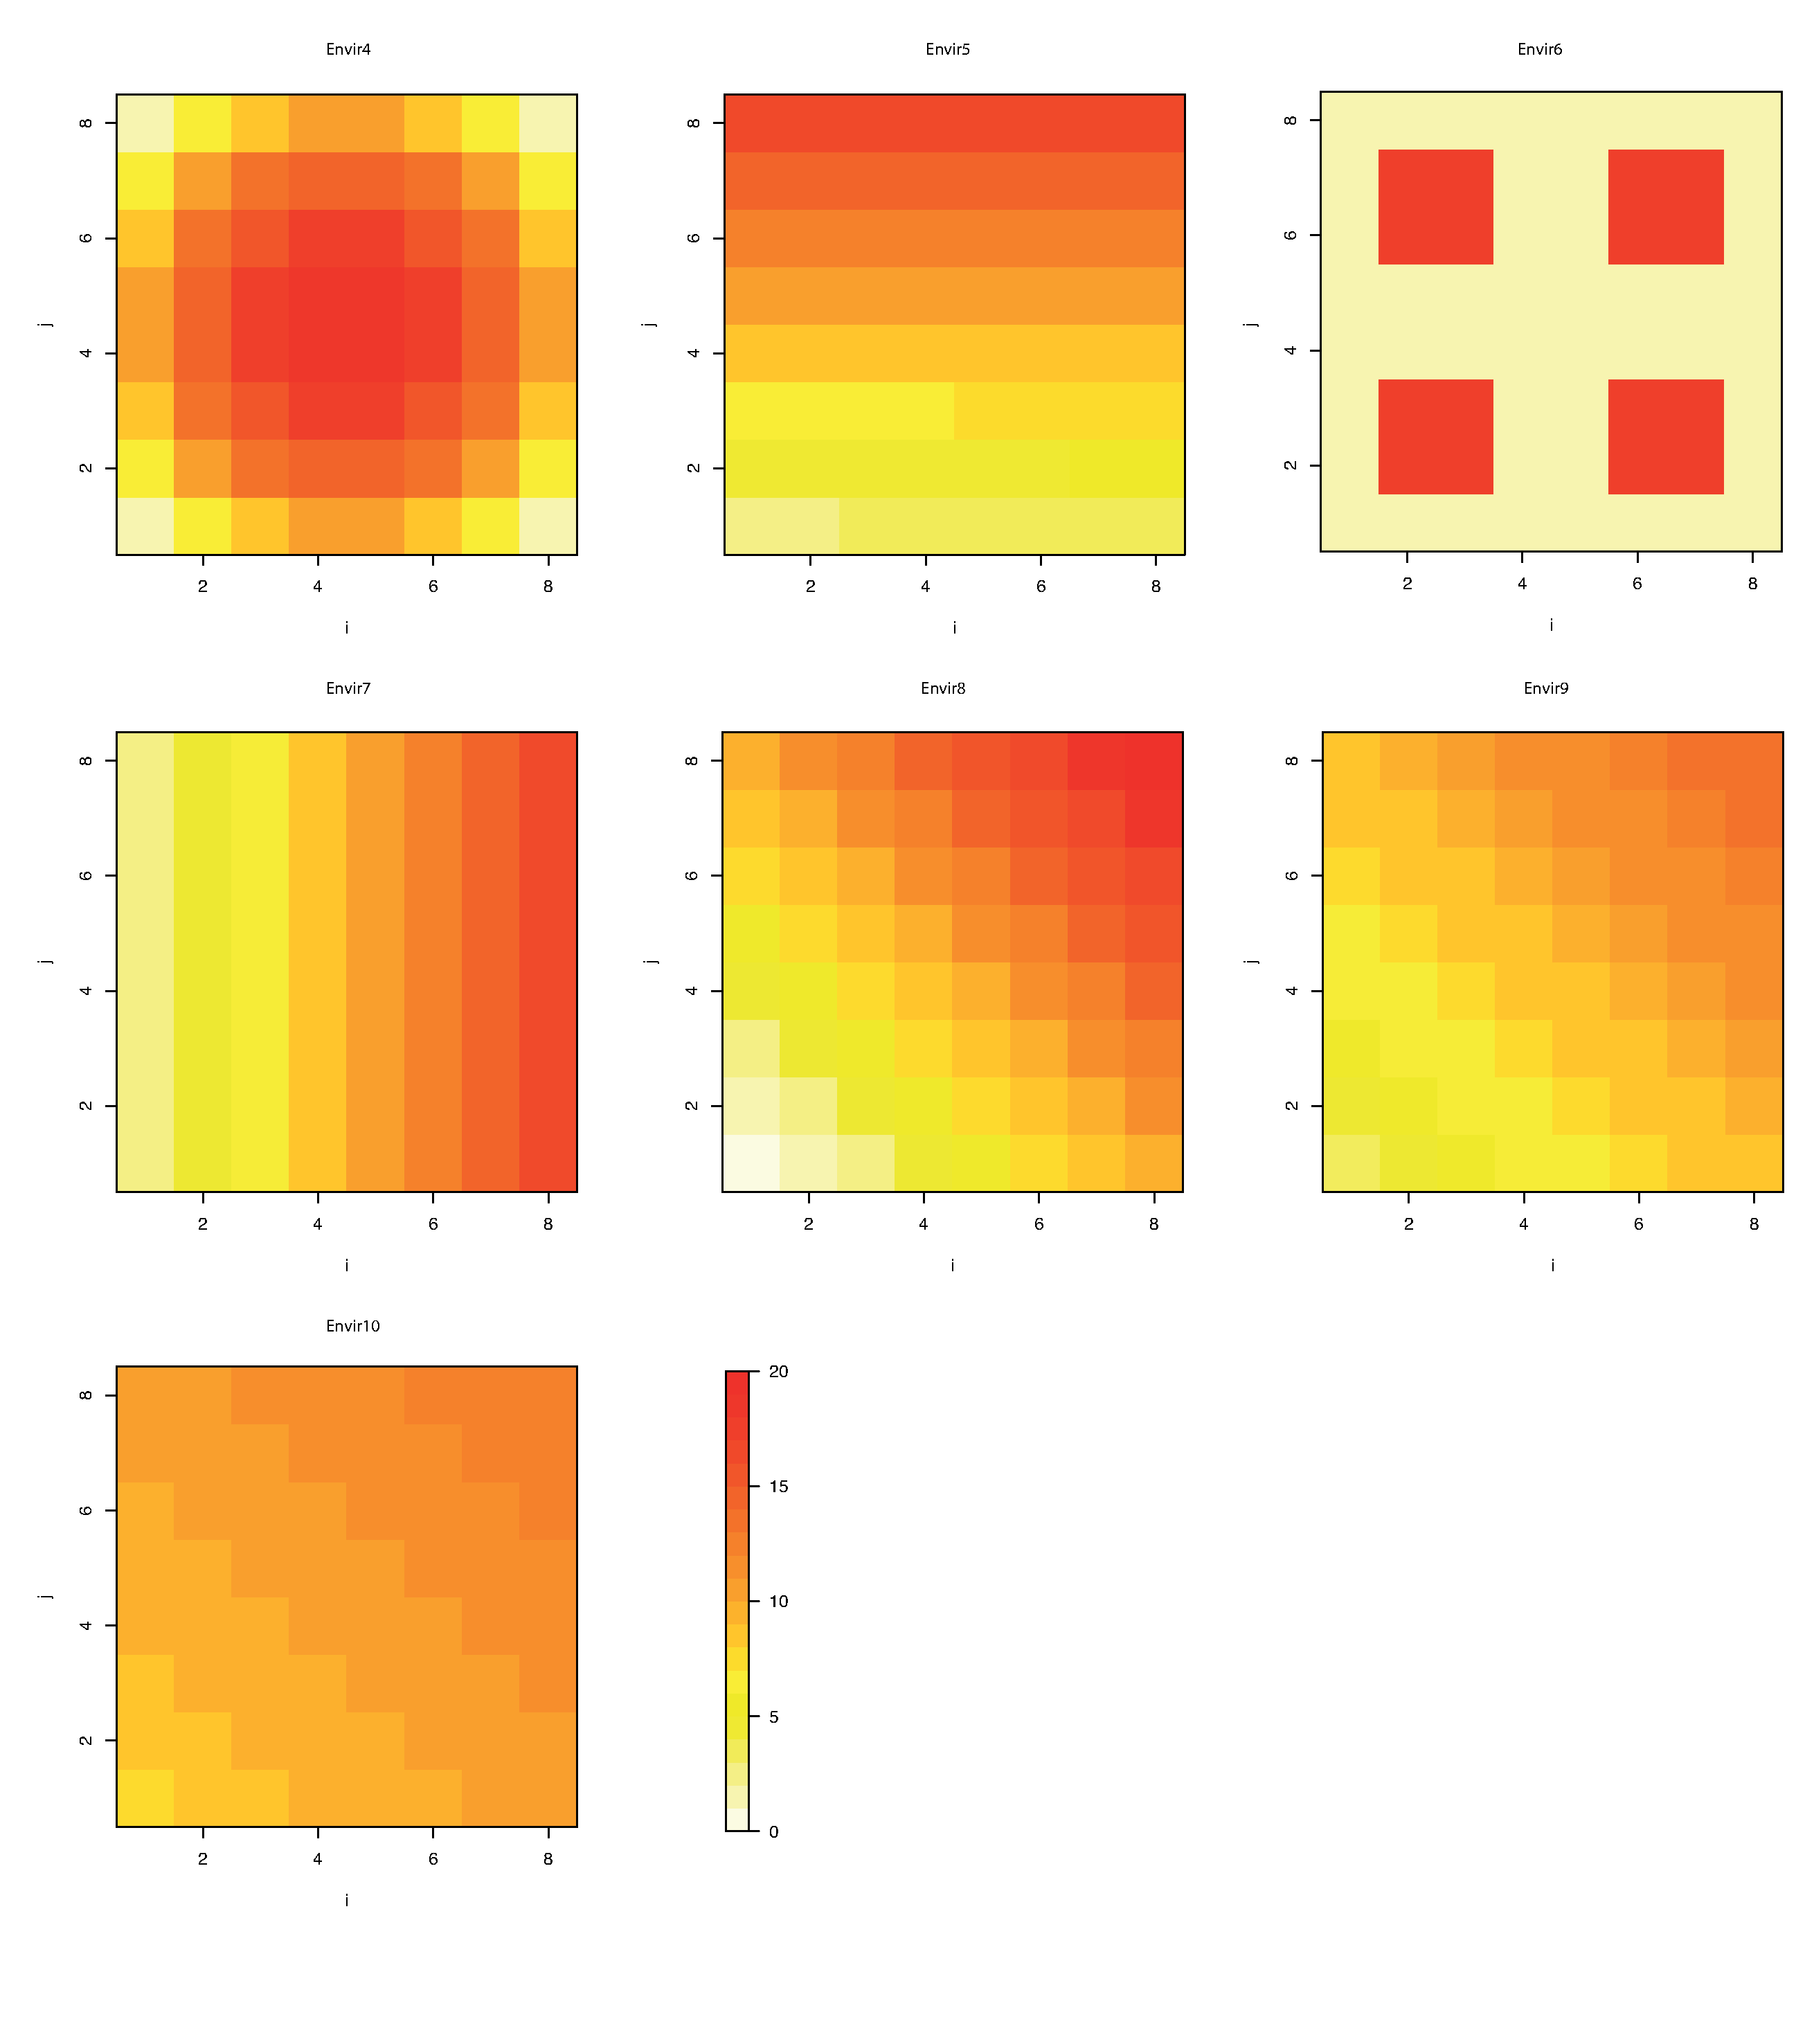
\includegraphics[height=0.8\textheight]{figures/environmentaldata.eps}
\end{center}
\caption{Graphical representation of mean environmental value for environment 4 to 10. Equation determining the environment is given in the main manuscript. Mean environmental value for environment 4, 5 and 6 are respectively equivalent to environment 1, 2 and 3.}%
\label{fig:environmentaldata}%
\end{figure*}


\begin{figure}[t]
\begin{center}
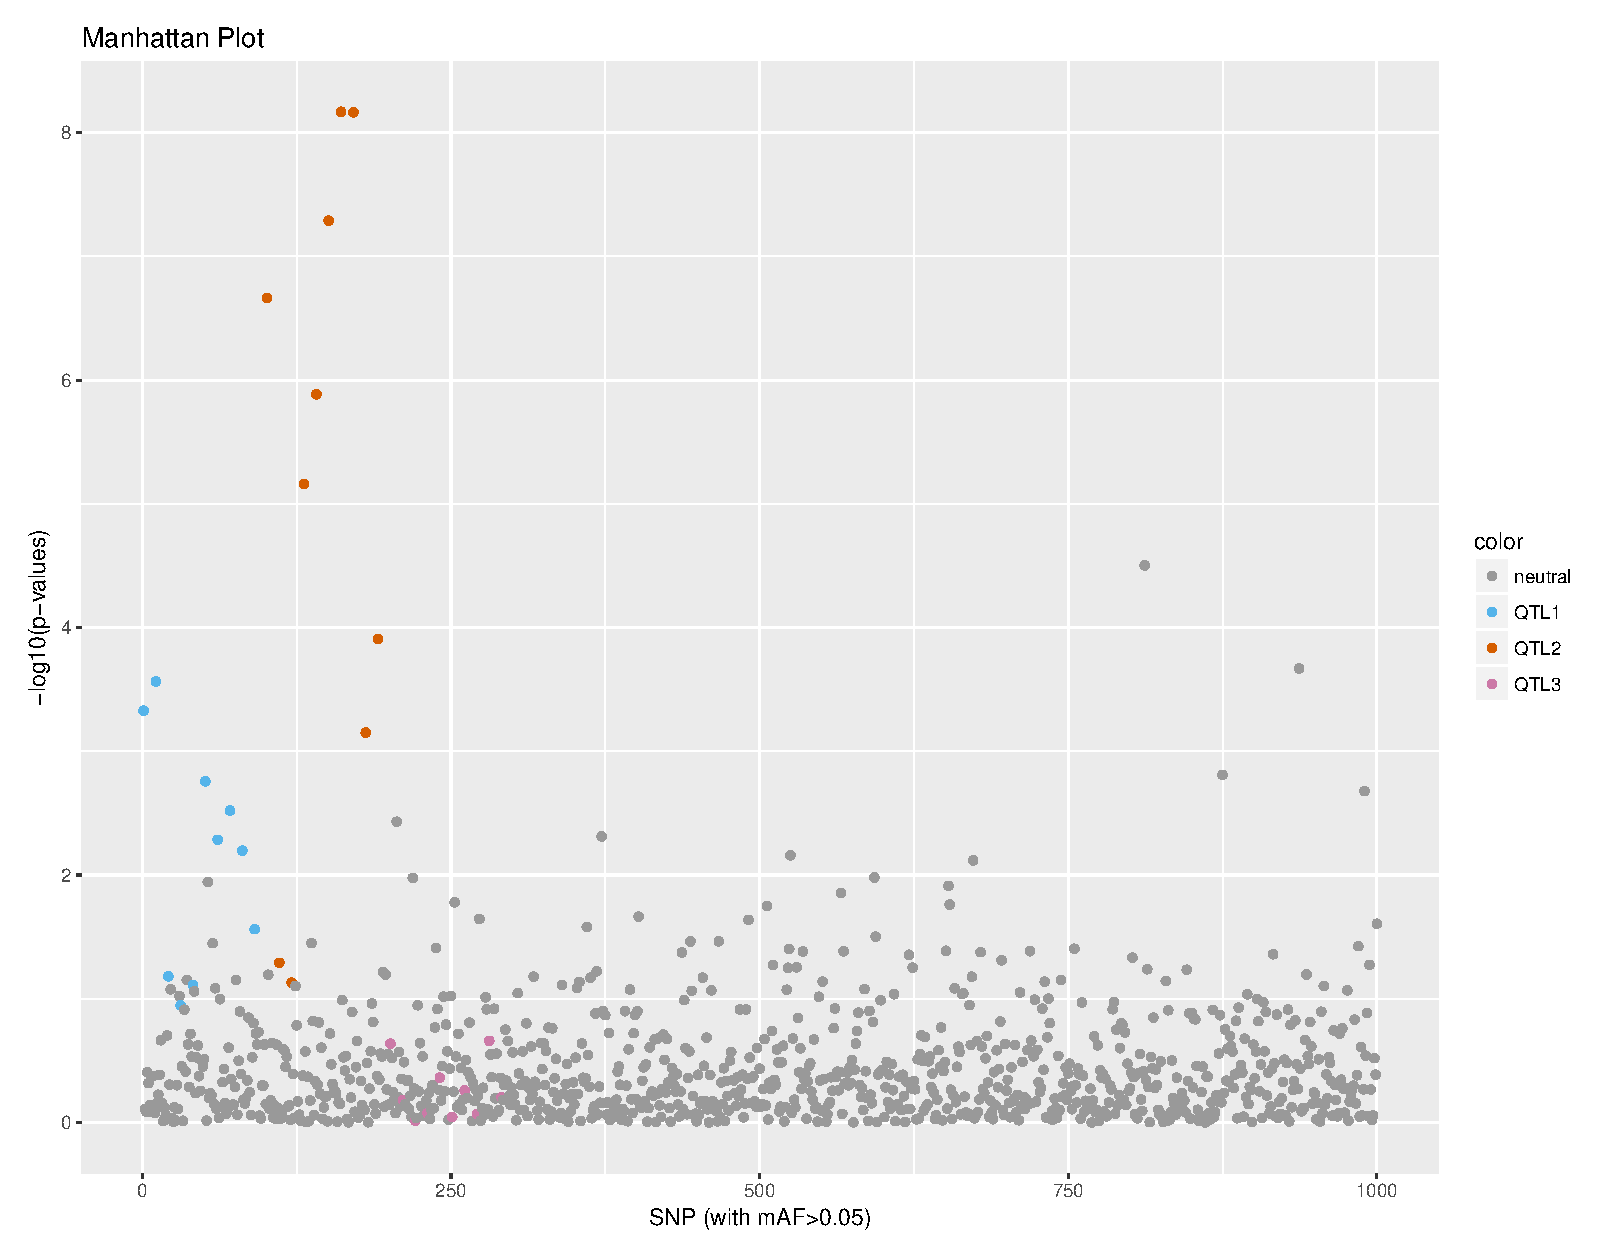
\includegraphics[height=0.4\textheight]{figures/sim105_pcadapt.eps}
\end{center}
\caption{Manhattan plot of the result of pcadapt on a simulated data set.}%
\label{fig:pcadapt}%
\end{figure}

\begin{figure}[t]
\begin{center}
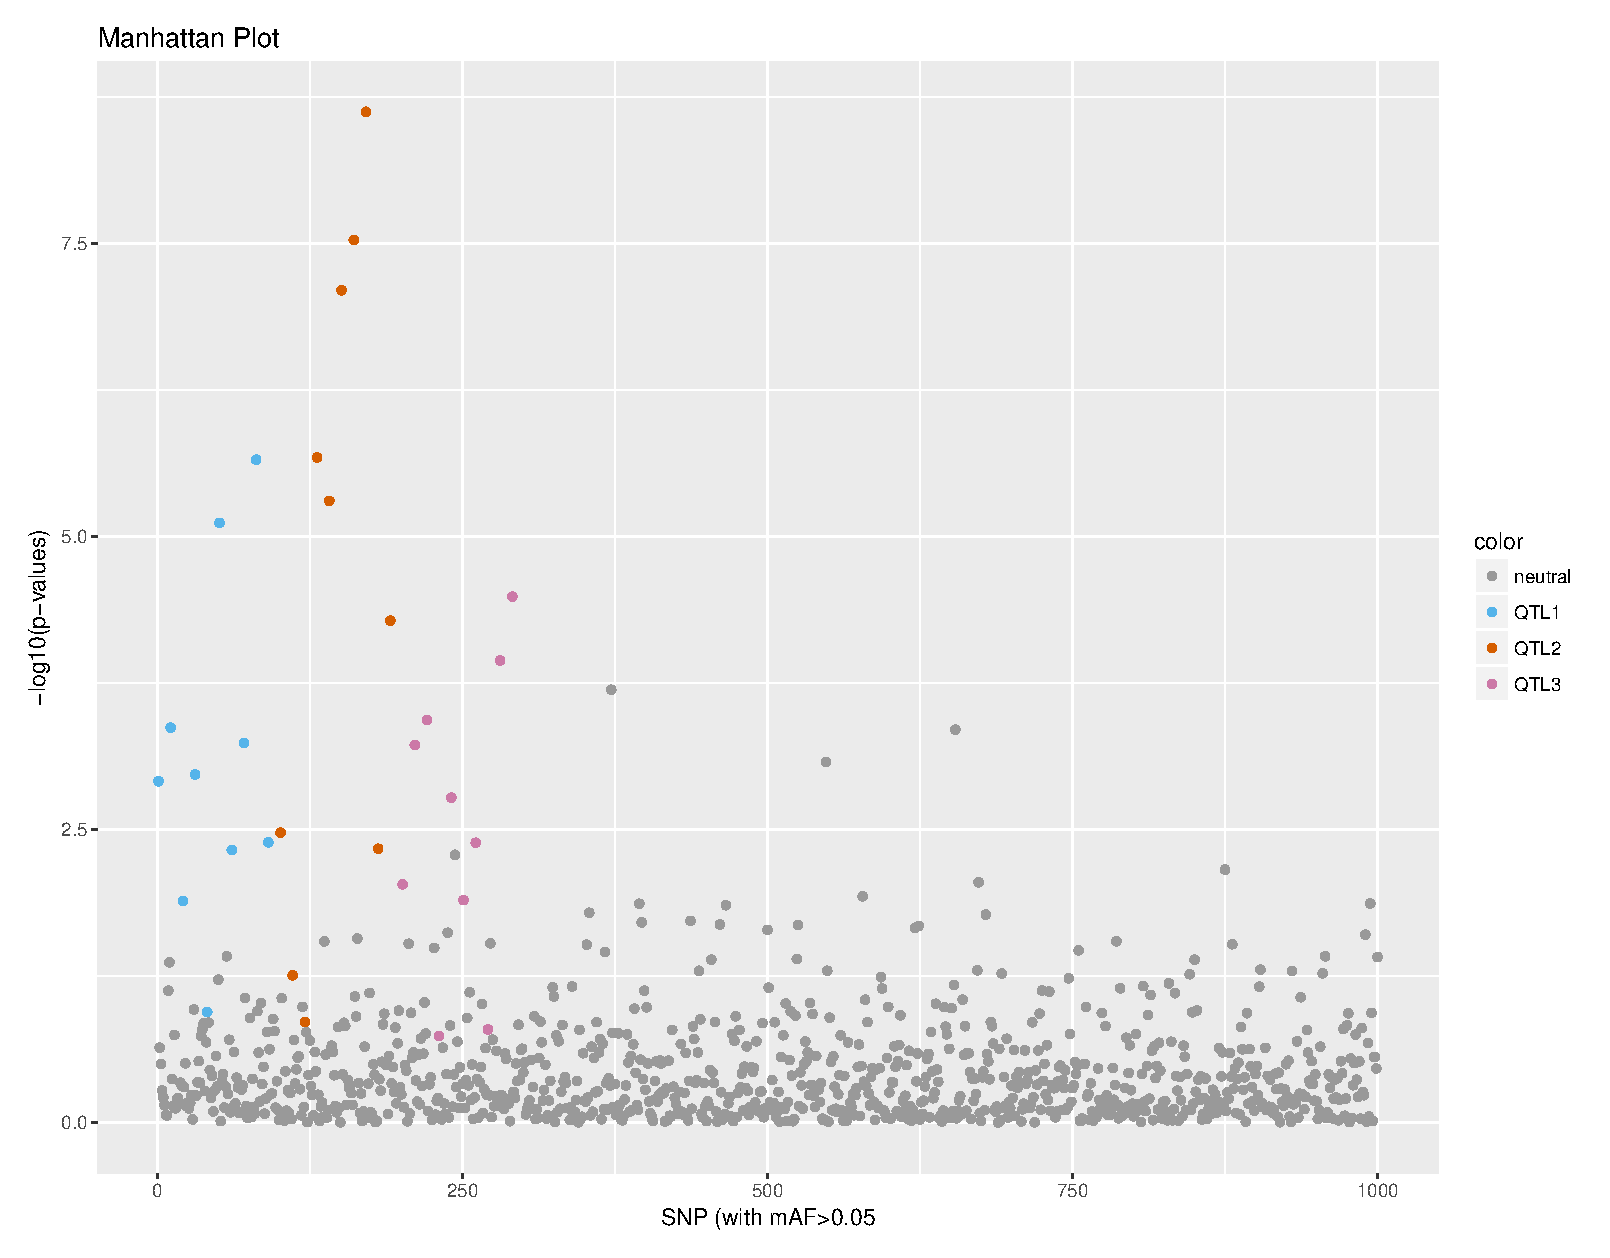
\includegraphics[height=0.4\textheight]{figures/sim105_capscale.eps}
\end{center}
\caption{Manhattan plot of the result of genome scan using RDA on a simulated data set.}%
\label{fig:rda}%
\end{figure}


\begin{figure*}[t]
\begin{center}
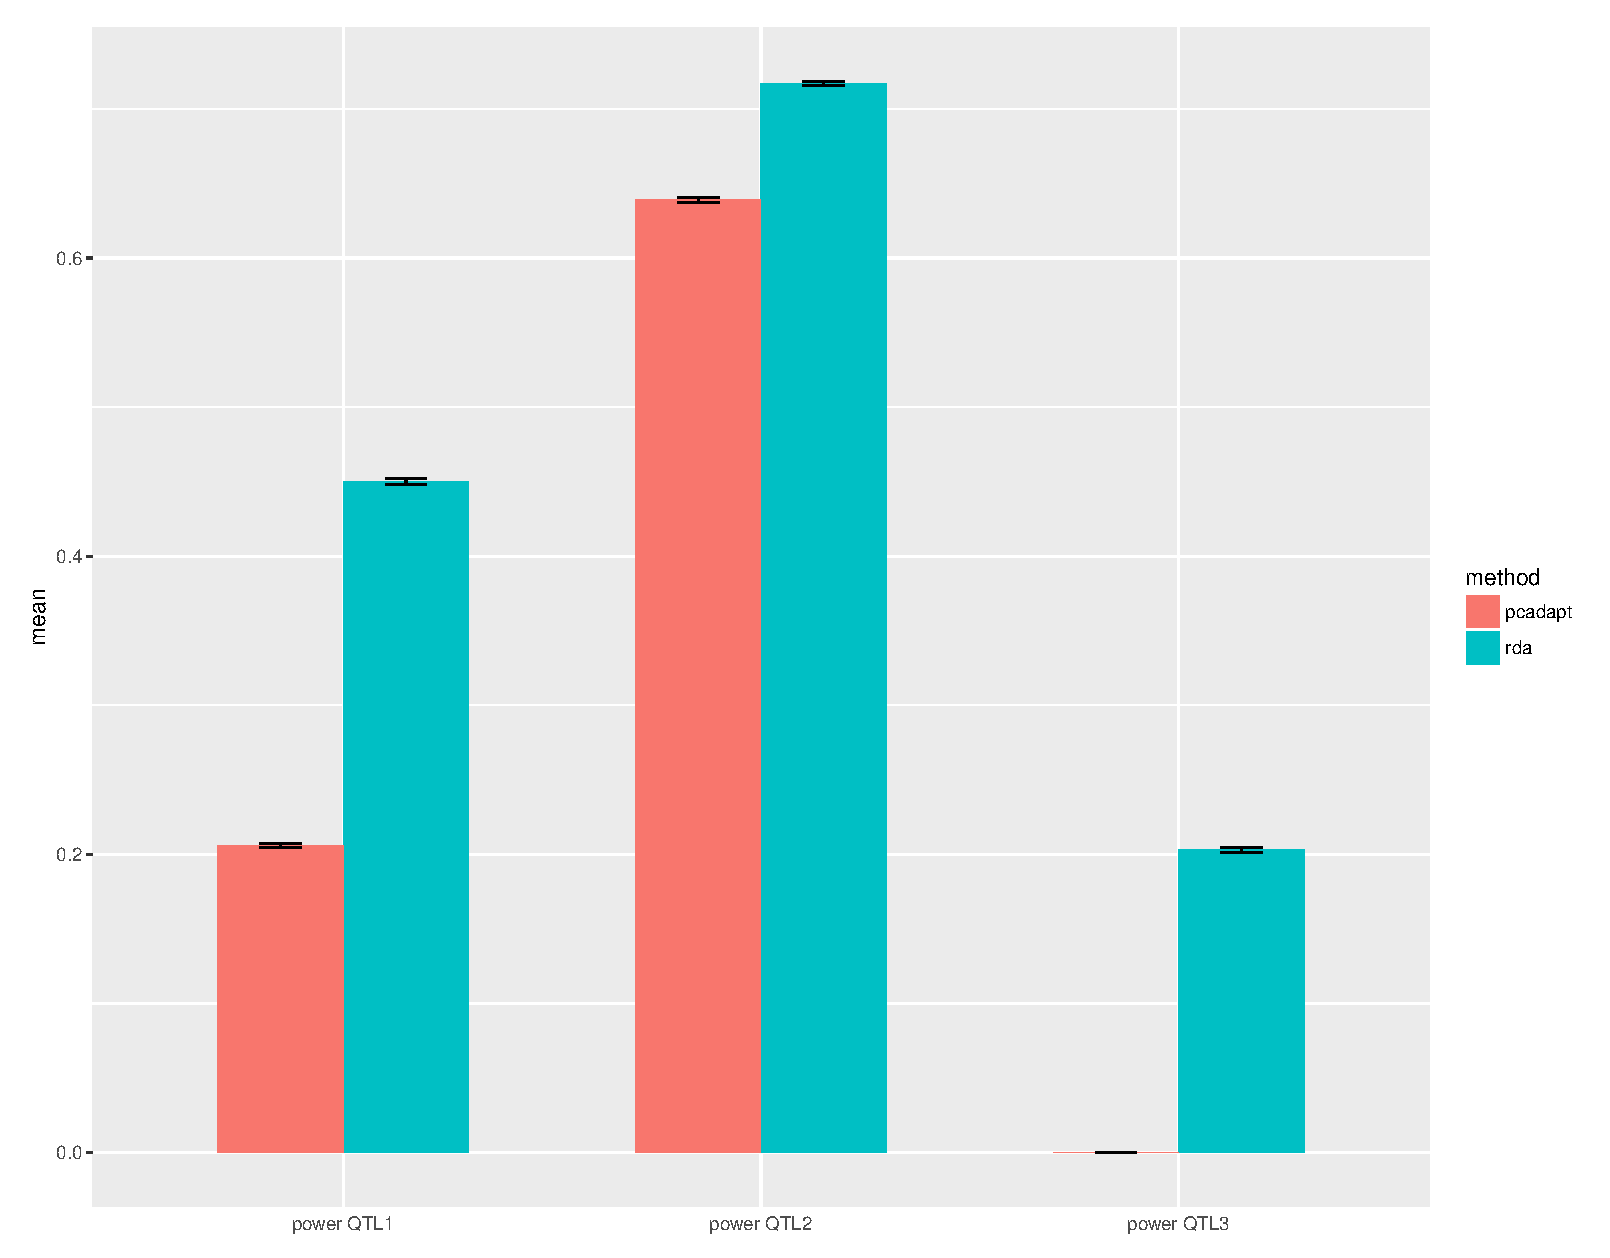
\includegraphics[height=0.4\textheight]{figures/overallresults.eps}
\end{center}
\caption{Performance results of rda and pcadapt methods. Each performance value is averaged over 100 simulated dataset (error bars are displayed but hardly visible since they are very scarce). Power is given seperately for loci coding for quantitative trait 1, 2 and 3.}%
\label{fig:performance}%
\end{figure*}

\begin{figure*}[t]
\begin{center}
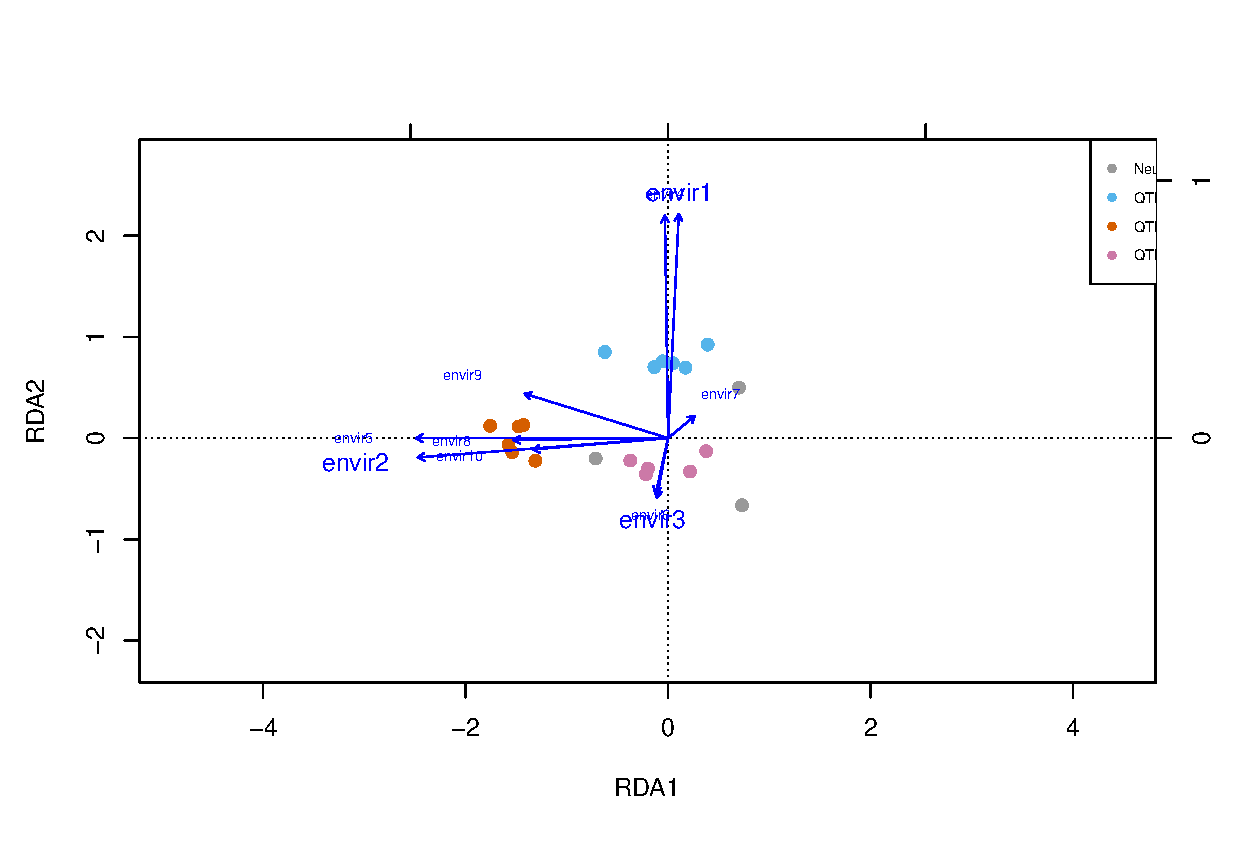
\includegraphics[height=0.4\textheight]{figures/rdaA.eps}
\end{center}
\caption{RDA on the adaptively enriched genetic space. We discarded the individual points for readability. Dots represents outliers SNPs.  $R^2$ of envir1 with the first, second and third axis is (0.172\%, 77.6\%, 17.6\%), envir2 is (94.5\%, 0.560\%, 0.236\%) and envir3 is (0.189\%, 5.34\%, 90.6\%)}%
\label{fig:rdaA}%
\end{figure*}

\begin{figure}[t]
\begin{center}
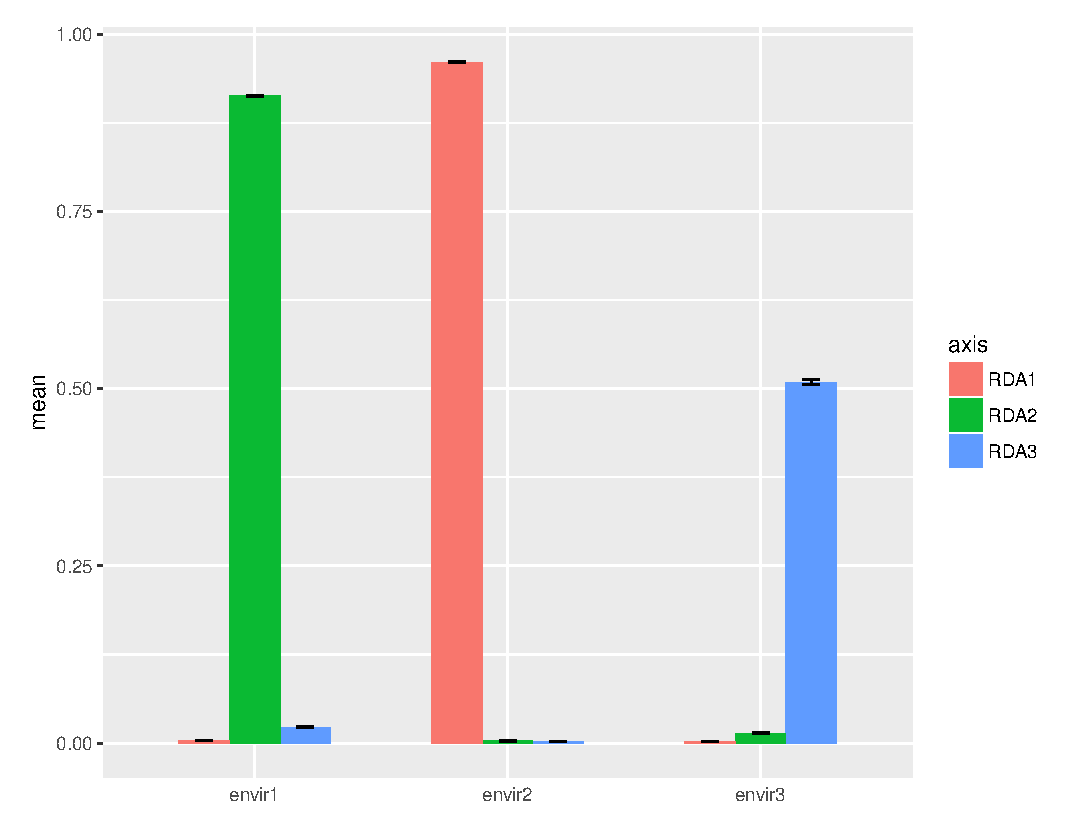
\includegraphics[height=0.4\textheight]{figures/R2.eps}
\end{center}
\caption{Percentage of variance explained by the first three ordination axis when the RDA is performed on all SNPs (red color) and when it is performed on the set of outliers loci (blue color). Values are averaged across the 100 simulated datasets.}%
\label{fig:R2}%
\end{figure}

\begin{figure*}[t]
\begin{center}
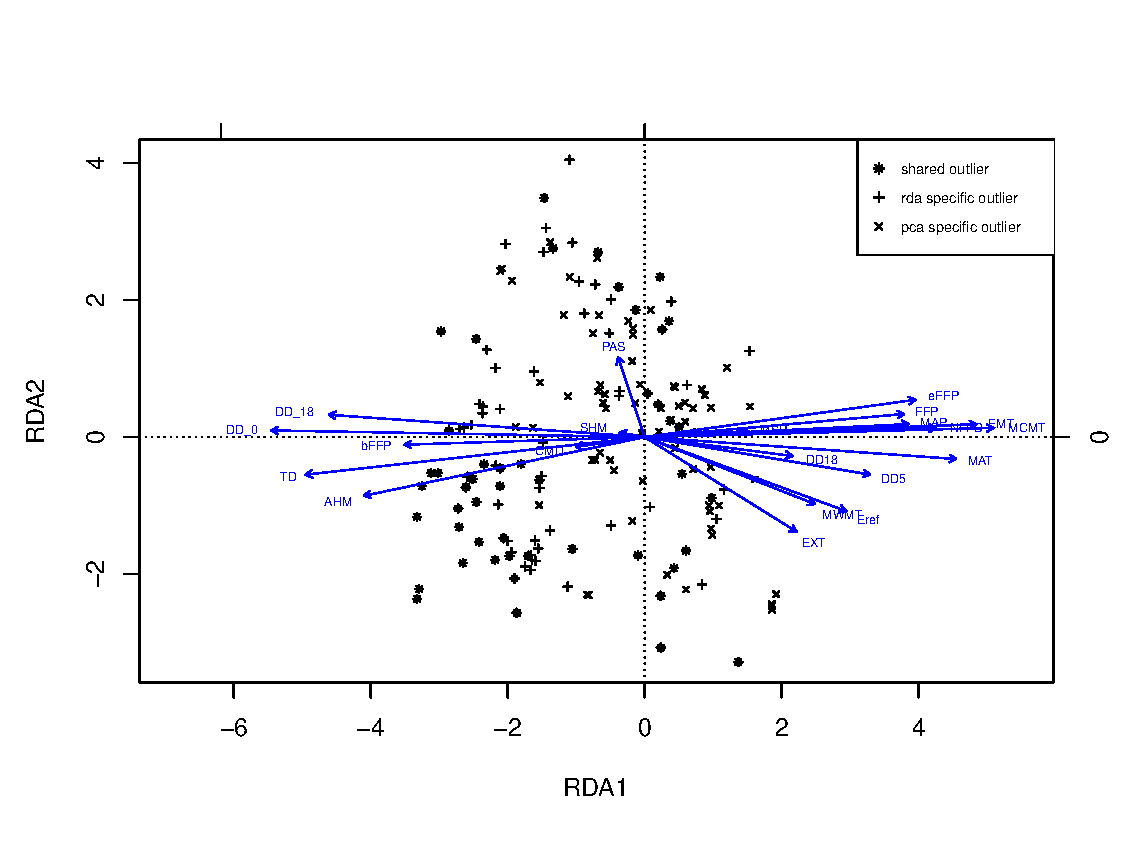
\includegraphics[height=0.4\textheight]{figures/poplar_rda.eps}
\end{center}
\caption{RDA on the adaptively enriched genetic space of \textit{P. trichocarpa} dataset (175 loci). We discarded the individual points for readability. Dots represents outliers SNPs either common or specific to RDA based genome scan and pcadapt.}%
\label{fig:poplar_rda}%
\end{figure*}

\begin{figure}[t]
\begin{center}
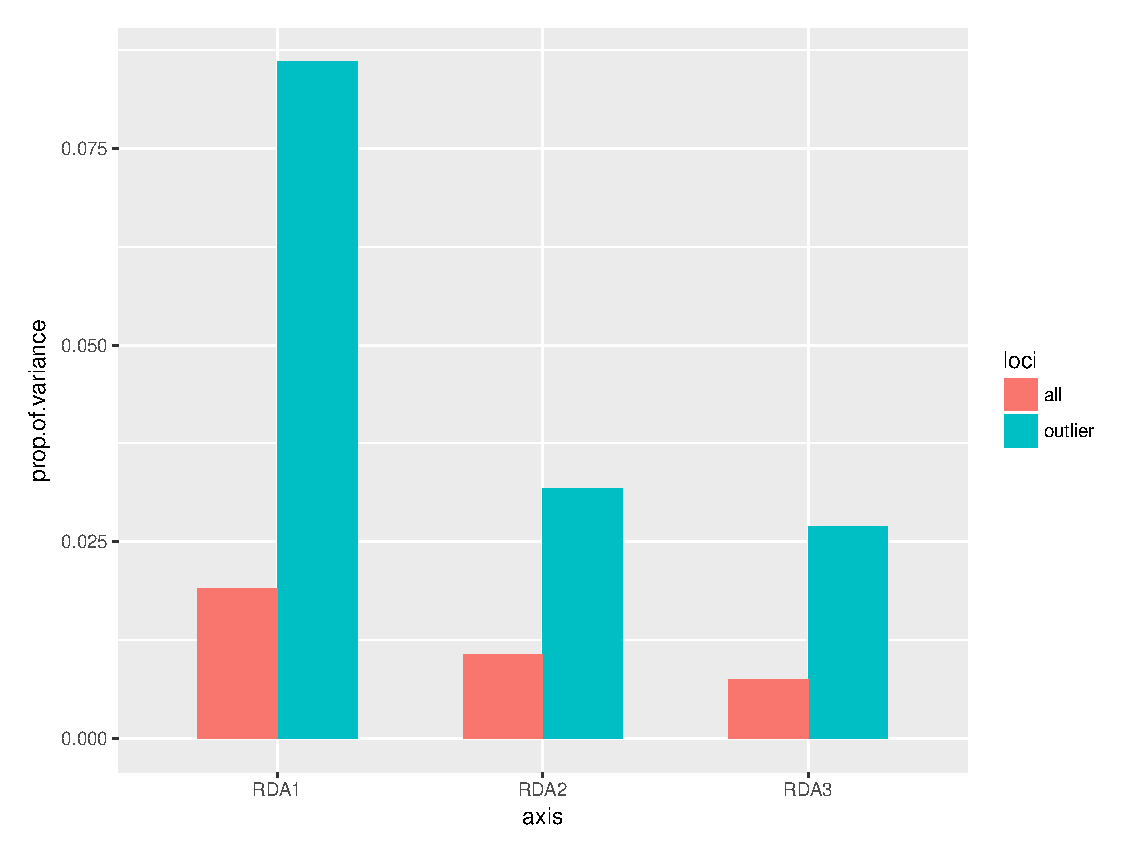
\includegraphics[height=0.4\textheight]{figures/varexplainedPopulus.eps}
\end{center}
\caption{Percentage of variance explained by the first three ordination axis when the RDA is performed on all SNPs (red color) and when it is performed on the set of outliers loci (175 loci - blue color).}%
\label{fig:varexplainedPopulus}%
\end{figure}



\end{document}